\documentclass[twocolumn]{article}
\usepackage[utf8]{inputenc}
% \documentclass[reprint, twocolumn]{revtex4-2} %formato

\counterwithout{figure}{section} % Si usas la clase 'article'
\usepackage{graphicx} % graficos
\usepackage{amsmath} %matrices
\usepackage{float}    
\usepackage{hyperref}


\graphicspath{{Imagenes/}} %graficos

\usepackage[spanish]{babel} %idioma

\usepackage{chngcntr}

\spanishdecimal{.}
\setlength{\parskip}{1em} 

\begin{document}

% \preprint{APS/123-QED}
\title{Modelamiento térmico, ajuste a la ley de Planck y caracterización de los elementos que componen  diferentes tipos de lámparas por medio del análisis de los espectros de emisión}
\author{Jesús Armando Cañas y Miguel Angel Perdomo }
% \affiliation{Universidad de Antiquia}
% \author{Miguel Angel Perdomo}
% \affiliation{Universidad de Antiquia}
\date{\today}

\maketitle
\begin{abstract}
    En el presente artículo se propone a realizar un ajuste a la ley de Planck con un estándar difuso, una esfera integradora y un espectroscopio, se verificó que este montaje sigue la ley de Planck y se analizó la temperatura de la lámpara por medio de la ley de Wein. En segundo lugar, se analizó los espectros de emisión de una lámpara de mercurio y argón, una lámpara fluorescente, un LED, para una pantalla LCD y una AMOLED, en el caso de las pantallas se analizó las diferencias entre sus espectro y cual presentaba un mejor rango cromático.
\end{abstract}
\section{Introducción}
Max Planck en 1901 formuló su famosa ley de la radiación del cuerpo negro o ley de Planck estableciendo que la energía se transmite por medio de paquetes de energía, es decir, de cuantos. Esta ley permitió describir la emisión de fuentes térmicas como las halógenas cuyo espectro es continuo y depende de la temperatura  sino que también sentó las bases para analizar espectros que no dependen de la temperatura. \cite{Planck1901}.

En general, se puede saber que elementos conforman un objeto sabiendo que tipo de luz emiten y a que intensidades, en general, fuentes de luz como las lámparas fluorescentes están conformadas por más de un elemento, en este caso en particular están compuestas por mercurio, argón y fosfatos \cite{Lamptech2011}, los primeros dos en estado gaseoso y los fosfatos en solido, esto debido a que el mercurio a ser excitado emite fotones en forma de rayos ultravioleta, el argón tiene la finalidad de hacer encender la lámpara más rápido \cite{moon1936scientific} y el fósforo cumple la función convertir la luz en forma de rayos ultravioletas a luz del espectro visible.

Teniendo en cuenta lo mencionado en los dos párrafos anteriores, se tiene como objetivo para este artículo realizar un ajuste a la ley de Planck de los datos obtenidos experimentalmente por medio de un espectrómetro, un estándar difuso y una esfera integradora, se comprobó que los datos seguían efectivamente la ley de Planck y se calculó la temperatura de la lámpara. En segundo lugar, se dispuso a analizar los espectro de una lámpara de mercurio-argón, una de lámpara fluorescente, de un LED, y de dos tipos de pantallas, una LCD y otra AMOLED, para ser posteriormente comparadas.

\section{Marco teórico}

\subsection{Excitación}
Cuando un electrón sufre un proceso de transición de un estado de energía a otro, se dice que sufre un proceso de des-excitación o excitación. Si el electrón se eleva por cualquier medio a un estado de energía
mayor, se dice que el átomo o el electrón están excitados. El átomo pierde la energía adquirida temporalmente, cuando el electrón regresa a un nivel más bajo y emite
energía radiante, un fotón cuya frecuencia es directamente proporcional a su energía\cite{Hewitt2007Conceptual}.

\[
E = hf
\]
\subsubsection{Espectros de emisión}
Todo elemento tiene una distribución característica de niveles electrónicos de
energía y, en consecuencia, emite luz con su propia distribución de frecuencias, es
decir, su espectro de emisión, cuando se excita\cite{Hewitt2007Conceptual}.

\subsection{Ley de Planck}
Un cuerpo negro es una sustancia capaz de absorber toda la radiación térmica que
incide sobre ella\cite{zemansky}. Sin embargo, emite radiación electromagnética en función de su temperatura y sirve para modelar la radiación térmica de otros objetos.

Planck consiguió modelar la curva de emisión de energía para un cuerpo negro, como una función que depende de la longitud de onda y de la temperatura del cuerpo negro \cite{Acevedo2021}.

\begin{equation}
    E(v,T)= \frac{2\pi h c^2}{\lambda^5}\frac{1}{e^{\frac{hc}{k_b \lambda T}}-1}
    \label{eq: Ley de planck}
\end{equation}

Donde:
\begin{itemize}
    \item $h$ : Constante de Planck.
    \item $c$ : Velocidad de la luz.
    \item $k_b$ : Constante de Boltzman.
\end{itemize}
\subsection{Ley de Wein}
La ley de desplazamiento de Wien permite obtener aquella longitud de onda donde la potencia de emisión es máxima y coincide con el máximo de emisión del modelo de Planck:
\begin{equation}
    \lambda_{max} = \frac{2898\mu m \cdot K}{T}
    \label{eq: ley de Wein}
\end{equation}


Se concluye que, a mayor temperatura de un cuerpo negro, menor es la longitud de onda en la que emite y, por tanto, mayor su frecuencia \cite{Acevedo2021}.

\subsection{Lámpara Fluorescente}
Una lámpara fluorescente simple consiste en dos cátodos en los extremos de un tubo que contiene gas de mercurio. Los cátodos distribuyen una corriente dentro del gas de mercurio; se produce una radiación ultravioleta cuando los electrones del cátodo desplazan los electrones del mercurio de su órbita natural (se excitan). Naturalmente, algunos de estos electrones volverán a su órbita natural liberando el exceso de energía absorbida durante la colisión (se desexcitan) en forma de radiación ultravioleta. Una modificación de la lámpara simple, las bombilla fluorescentes (incluyendo las fluorescentes compactas o CFL), cuentan además con una capa de fósforo en la superficie del tubo que permite convertir esa luz ultravioleta en luz del espectro visible, fenómeno denotado por fluorescencia~\cite{singh2013comparative}. Adicionalmente, para mejorar su eficiencia se suelen usar gases como el argón o el neón para facilitar el encendido de la lámpara~\cite{moon1936scientific}. El fósforo empleado para estas lámparas actualmente consta de varios elementos de tierras raras para mejorar su calidad de luz \cite{Lamptech2011}.

\subsection{Diodos Emisores de Luz (LEDs)}
Un diodo emisor de luz, es un diodo que con un espacio en la unión P-N. El led emite luz cuando pasa corriente del ánodo al cátodo de la unión P-N del dispositivo. Se requiere una fuente de corriente continua (CC) para su alimentación. Por otro lado, debe aplicarse un voltaje umbral lo suficientemente alto como para que el led funcione. La corriente que pasa por el diodo genera un exceso de electrones (portadores de carga negativa) en la capa de transporte y huecos (portadores de carga positiva) en la capa de transporte del diodo que posteriormente se combinan en la unión P-N ,por lo tanto, este exceso de energía se convierte en luz~\cite{singh2013comparative}.

\subsection{Pantalla de cristal líquido (LCD)}

\subsubsection{Cristal líquido}
Los cristales líquidos son materiales que presentan propiedades tanto de líquidos como de sólidos, se pueden considerar como una fase intermedia. Estos materiales pueden ser clasificados como nemático, esméctico y coléstrico. En este artículo, solo se explicará los nemáticos pues son los cristales líquidos que más comúnmente se emplean para la fabricación de las pantallas LCD debido a sus propiedades físicas. En particular, las moléculas de estos cristales están orientadas en promedio de una forma específica, al aplicarse un campo eléctrico o magnético la orientación de las moléculas podrá ser manipulada de forma predecible, lo cual, lo hace útil para las pantallas LCD~\cite{gurski2005display}.

\subsubsection{Lentes Polarizadores}
Un polarizador es aquel material que solo permite que los campos eléctricos y magnéticos de una onda de luz pasen por un solo plano, todas las componentes que estén por fuera son absorbidas. Si se considera dos lentes polarizadores, con la segunda con un desfase de 90°, al pasar la luz por la primera lente, solo pasará la luz en un solo plano, al pasar por el segundo, no pasará nada de luz~\cite{gurski2005display}.

\subsubsection{Modos de transmisión de Luz}
Las pantallas LCDs no emiten su propia luz, por lo cual, cuentan con tres tipo de transmisión de luz: reflectiva, transmisiva y transflectiva. Ésta última es la que se emplea en las pantallas LCD de los teléfonos inteligentes, así que se hará un énfasis en ella. En el fondo de la pantalla, tras el cristal líquido existe una fuente de iluminación uniforme que permite que la pantalla LCD emita colores y se vean incluso a plena luz del día~\cite{gurski2005display}.

\subsubsection{Matriz Activa}
En una pantalla LCD más compleja (como la de los celulares), cada pixel (es decir, cada unidad mínima direccionable de una pantalla compuesta por tres colores primarios: verde, rojo y amarillo) tiene un transistor que permite controlar la cantidad de carga que recibe un píxel; es decir, así se permite controlar su intensidad y color con mucha precisión. Además, para cada pixel se tiene un pequeño capacitor en paralelo que permite que cada píxel permanezca por un corto periodo de tiempo en el mismo color e intensidad hasta el siguiente ciclo de actualización, evitando que la pantalla parpadeé~\cite{gurski2005display}.
\subsection{Pantallas de diodos orgánicos emisores de luz (OLEDs)}
Los diodos orgánicos emisores d luz son como dice su nombre, un material orgánico emisor de luz, intercalado entre dos placas conductoras, una de material tipo n y otra de tipo p. En la estructura del material tipo n a pesar de ser neutra tiene un electrón extra que puede ser movido del material con relativa facilidad. En el material tipo p ocurre lo contrario, hay un hueco donde un electrón puede moverse libremente. Al aplicarse un voltaje entre las dos placas se inyectan huecos en la placa tipo p y electrones en la tipo n, cuando un electrón llena un hueco, desciende a un nivel de energía inferior; por lo tanto, libera esa diferencia de energía como un fotón~\cite{gurski2005display}.

\subsubsection{Pantallas de matriz activa (AMOLED)}
A comparación de una pantalla de matriz pasiva donde la corriente se distribuye secuencial mente fila por fila, las pantallas de matriz activa usan transistores TFT para tener un control individual de cada pixel, cada pixel es gestionado por dos TFTs: el primero actúa como interruptor para cargar un capacitor y el segundo establece una fuente corriente constante para mantener la iluminación de ese pixel~\cite{gurski2005display}.

\subsection{Calibración del espectrómetro}
El estándar principal para la escala de radiancia espectral, mantenida en la Instalación de Calibraciones Espectrorradiométricas Automatizadas (FASCAL) del Instituto Nacional de Estándares y Tecnología, es un cuerpo negro que opera a la temperatura de congelación del oro \cite{Early1996Irradiance}, cuya distribución espectral está dada por la ecuación \ref{eq: Ley de planck}.

La manera en la que se calibran los espectrómetros digitales para aquellos detectores que presentan respuestas con comportamientos lineales, viene dada por la ecuación:
\[
    S(\lambda)= E(\lambda)\cdot R(\lambda) + D(\lambda)
\]

$S(\lambda)$ es la señal medida por el detector del espectrorradiómetro, $E(\lambda)$ es la irradiancia espectral de la lámpara, $R(\lambda)$ es la respuesta a la irradiancia espectral del espectrorradiómetro y $D(\lambda)$ es la señal medida en oscuridad. \cite{Rammeloo2023Spectroradiometer}
Si se linealiza y normaliza la ecuación anterior, se obtiene la siguiente ecuación:
\begin{equation}
    E_{\lambda}= B_{\lambda}(\frac{S_{\lambda}-D_{\lambda}}{R_{\lambda}-D_{\lambda}})
    \label{eq: ecuación de transferencia radiométrica relativa}
\end{equation}


\subsection{Bondad de ajuste y test de hipótesis}

Inicialmente, una hipótesis es aquella suposición que se plantea respecto a alguna población o problema con el fin de verificar su veracidad o falsedad. Adicionalmente, una hipótesis nula $H_0$ es aquella hipótesis que inicialmente se asume como cierta con la finalidad de verificarla o falsarla, y la hipótesis alternativa $H_a$ será una suposición que sea contraria a la hipótesis nula. Cabe aclarar que tanto la hipótesis nula como la alternativa deben ser mutuamente excluyentes (contrarias entre sí). Se le llama test de hipótesis a aquel proceso mediante el cual se busca aceptar o rechazar la hipótesis nula. Sin embargo, cabe añadir que este es un proceso probabilístico y no absoluto; por lo cual, que la hipótesis nula sea verdadera o falsa no es un hecho inequívoco. Para poder verificar o falsar la hipótesis nula, existen múltiples herramientas, como la llamada \textit{prueba de bondad de ajuste}, con la cual podemos determinar si ciertos datos experimentales se ajustan a una distribución determinada \cite{marques1991probabilidad}.

\subsection{Matriz de Covarianza}\label{covarianza}
La covarianza es una medida que indica el grado en que dos variables aleatorias varían conjuntamente.

Para dos variables aleatorias $X$ y $Y$, la covarianza se define como:

\begin{equation}
\mathrm{Cov}(X,Y) = E[(X - \mu_X)(Y - \mu_Y)]
\end{equation}

donde $\mu_X$ y $\mu_Y$ son las medias de $X$ y $Y$, respectivamente.

Para un conjunto de datos muestrales, la covarianza se calcula mediante la siguiente expresión:

\begin{equation}
\mathrm{Cov}(X,Y) = \frac{1}{n} \sum_{i=1}^{n} (x_i - \bar{x})(y_i - \bar{y})
\end{equation}

La matriz de covarianza para un vector aleatorio $\mathbf{X} = (X_1, X_2, \dots, X_p)$ se define como:

\begin{equation}
\begin{pmatrix}
\mathrm{Var}(X_1) & \mathrm{Cov}(X_1,X_2) & \cdots & \mathrm{Cov}(X_1,X_p) \\
\mathrm{Cov}(X_2,X_1) & \mathrm{Var}(X_2) & \cdots & \mathrm{Cov}(X_2,X_p) \\
\vdots & \vdots & \ddots & \vdots \\
\mathrm{Cov}(X_p,X_1) & \mathrm{Cov}(X_p,X_2) & \cdots & \mathrm{Var}(X_p)
\end{pmatrix}
\end{equation}

donde los elementos de la diagonal representan las varianzas y los elementos fuera de la diagonal representan las covarianzas.

Esta matriz es simétrica y juega un papel fundamental en el análisis multivariado y en la teoría de regresión~\cite{marques1991probabilidad}.

\subsection{Incertidumbres pequeñas} \label{Inceridumbres pequeñas}
Sea $x$ una variable aleatoria, tal que $x=f(u,v,\dots)$. Luego, su varianza $\sigma_x^2$ se puede determinar como~\cite{bevington2003data}:

\begin{equation}
    \sigma_x^2=\sigma_u^2\left(\frac{\partial x}{\partial u}\right)^2 + \sigma_v^2\left(\frac{\partial x}{\partial v}\right)^2 + \dots + 2\sigma_{uv}^2\left(\frac{\partial x}{\partial u}\right)\left(\frac{\partial x}{\partial v}\right)
\end{equation}

\subsection{Distribución chi-cuadrado}
\label{seccion chi}
Si se considera que ciertos datos siguen una distribución determinada, se puede establecer que un evento $E_k$ ocurre con una frecuencia observada $O_k$. Según la distribución teórica, los datos siguen una frecuencia esperada $e_k$; luego, $\chi^2$ se define como \cite{marques1991probabilidad}:

\begin{equation}
\chi^2 = \sum_{k=1}^{n} \frac{(O_k - e_k)^2}{e_k} 
\label{chi}
\end{equation}

Finalmente, tras obtener el estadístico de la distribución chi-cuadrado, es necesario considerar cómo se va a concluir y bajo qué condiciones se determinará que la hipótesis nula se cumple. Así, se define el nivel de significancia ($\alpha$) como la probabilidad de rechazar la hipótesis nula aunque esta sea cierta. Usualmente, en física experimental se emplea un nivel de significancia igual al 5\% \cite{marques1991probabilidad}.
\subsection{Grados de libertad y valor crítico}
Los grados de libertad de una distribución pueden calcularse como~\cite{sirca2016probability}:
\begin{equation}
    \nu = n - m - 1 
 \label{eq: grados de libertad}
\end{equation}
Donde cada término se define de la siguiente manera:

\begin{itemize}
    \item[$n$:] Número de clases o bines independientes en los que se han agrupado los datos del histograma.
    \item[$m$:] Número de parámetros que no son conocidos a priori y que se estiman mediante los datos obtenidos experimentalmente~\cite{sirca2016probability}.
\end{itemize}

Por otro lado, el valor crítico se define como aquel umbral tal que, si el estadístico chi-cuadrado es mayor que dicho valor, se rechaza la hipótesis nula; de lo contrario, si es menor, la hipótesis nula es aceptada. A partir del nivel de significancia, se puede calcular el valor crítico ($x_*$) como~\cite{sirca2016probability}:

\begin{equation}
    \alpha = \int_{x_*}^{\infty} f(x; \theta_0) \, dx 
\end{equation}

\begin{tabular}{p{7cm} p{5.5cm}}
    $x_*$: Valor crítico.\\
    $f(x;\theta)$:
    Función de densidad de probabilidad del estadístico de prueba bajo la hipótesis nula, caracterizada por el parámetro $\theta$.\\
    $\alpha$: Nivel de significancia.
\end{tabular}

\subsection{Error porcentual $\epsilon_{\%}$}
Si se tiene un valor aceptado de una constante ($v_a$) y un valor experimentalmente obtenido ($v_e$), el error porcentual $\epsilon_{\%}$ se determina como~\cite{JCGM2008}:

\begin{equation}
    \epsilon_{\%} = \frac{|v_a - v_e|}{v_a} \times 100\%
    \label{eq: error porcentual}
\end{equation}
\section{Metodología}

\subsection{Montaje}
A continuación se muestra el montaje empleado durante el experimento:


\begin{figure}[ht]
     \centering
     \includegraphics[width =1 \linewidth]{foto montaje actividad 4.jpg}
     \caption{Representación gráfica del número de conteos de intensidades para el test de $\chi^2$}
     \label{fig: foto montaje}
\end{figure}

En el lado izquierdo de la figura \ref{fig: foto montaje} se puede observar al espectrómetro digital Thorlabs CCS100 conectado a una fibra óptica (cable azul), al lado izquierdo y conectado al espectrómetro se encuentra el computador desde donde se procesarán los datos para su posterior análisis. 

\subsection{Etapa 1}

\begin{figure}[H]
     \centering
     \includegraphics[width =1 \linewidth]{Imagenes/esfera integradora.jpg}
     \caption{Representación gráfica del número de conteos de intensidades para el test de $\chi^2$}
     \label{fig: esfera integradora}
\end{figure}

En la primera etapa, se conectó a la esfera integradora de la figura \ref{fig: esfera integradora} la fibra óptica de la figura \ref{fig: foto montaje} (cable azul). Posteriormente, se procedió a medir el espectro con la esfera integradora encendida y el estándar difuso, luego se midió el espectro sin el estándar y con esfera integradora encendida, por último, se midió el espectro con la lámpara apagada y sin el estándar. 

Después, empleando la ecuación \ref{eq: ecuación de transferencia radiométrica relativa} se calculo la radiancia. Luego, se realizó a los datos un ajuste a la ley de Planck, de la forma:

\begin{equation}
        E= \frac{A}{\lambda^5}\frac{1}{e^{\frac{B}{ \lambda }}-1}
    \label{eq: Ajuste ley de planck}
\end{equation}

A partir del parámetro $B$ se calculó la temperatura $T$ mediante la siguiente expresión:

\begin{equation}
    T = \frac{10^{9}h c}{k_b B}
    \label{eq :temperatura}
\end{equation}

Cuya incertidumbre se determinó con la matriz de covarianza del ajuste (sección \ref{covarianza}), y por medio de la propagación de incertidumbres pequeñas (sección \ref{Inceridumbres pequeñas}) que corresponde a la siguiente expresión:

\begin{equation}
    \Delta T = \frac{10^{9}h c}{k_b B^2} \cdot \sigma_{11}
    \label{eq: pequeñas incertidumbres}
\end{equation}

Por último, se realizó una prueba de bondad de ajuste para verificar que los datos obtenidos siguen el ajuste. Se toma a $H_0$ como: \textit{Los datos experimentales siguen la ley de Planck}, y a $H_a$ como: \textit{Los datos experimentales no siguen la ley de Planck}. Extrapolando el ajuste obtenido hasta los $6000 \,nm$, se determinó el valor de $\lambda$ que correspondía al pico máximo del espectro extrapolado, para calcular la temperatura a partir de la ecuación \ref{eq: ley de Wein}. Con respecto a este valor, se calculó el error porcentual del valor de temperatura obtenido con el parámetro de ajuste.

\subsection{Etapa 2}
En esta etapa se midió el espectro de una lámpara de mercurio - argón, una lámpara fluorescente, una lámpara led, de una pantalla LCD y una pantalla AMOLED. El procedimiento consistió en tomar cada fuente de luz, acercarla a la fibra óptica (cable azul) de la imagen \ref{fig: foto montaje}, extraer los datos proporcionados por el espectrómetro y realizar un análisis cualitativo de los mismos .En el caso de la lámpara de mercurio-argón, se identificó a qué elemento correspondía cada línea del espectro de emisión. De manera análoga, se realizó este análisis para la lámpara fluorescente. Finalmente, para la lámpara LED y las pantallas AMOLED y LCD, se estudió el origen de las formas características presentes en sus respectivos espectros de emisión.

\section{Resultados}
\subsection{Ajuste de la ley de planck}
% \begin{figure}[H]
%     \centering
%     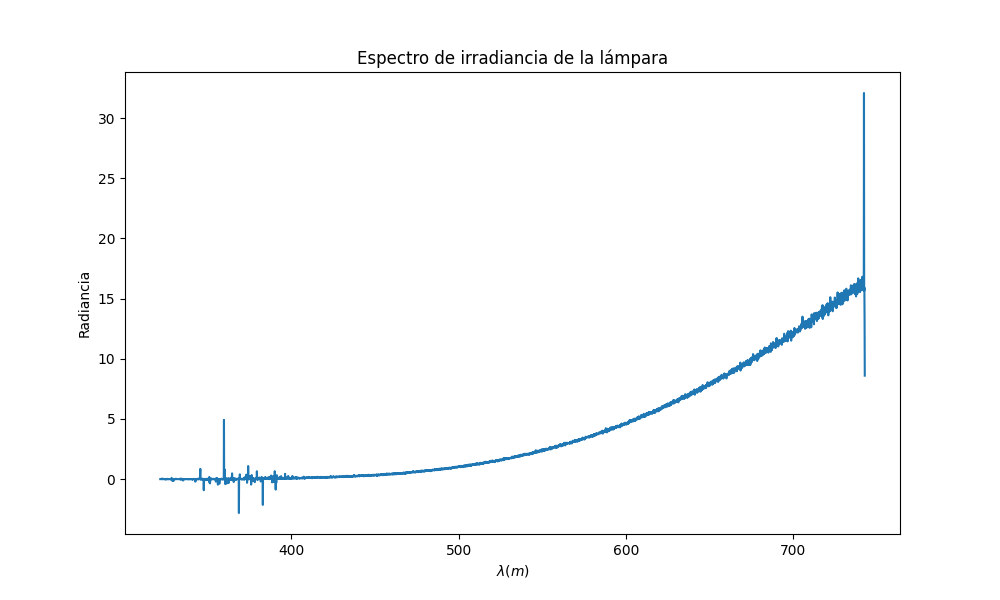
\includegraphics[width =1\linewidth]{Espectro_de_irradiancia_de_la_lampara.png}
%     \label{fig: ley de planck}
%     \caption{Datos del espectro de irradiancia}
% \end{figure}
Al aplicar la ecuación \ref{eq: ecuación de transferencia radiométrica relativa} a los datos de la primera etapa. Se obtuvo el comportamiento de la intensidad ($I$) en función de la longitud de onda ($\lambda$) mostrado en la gráfica 1, de la figura \ref{fig: Ajuste de la ley de planck}


\begin{figure}[H]
    \centering
    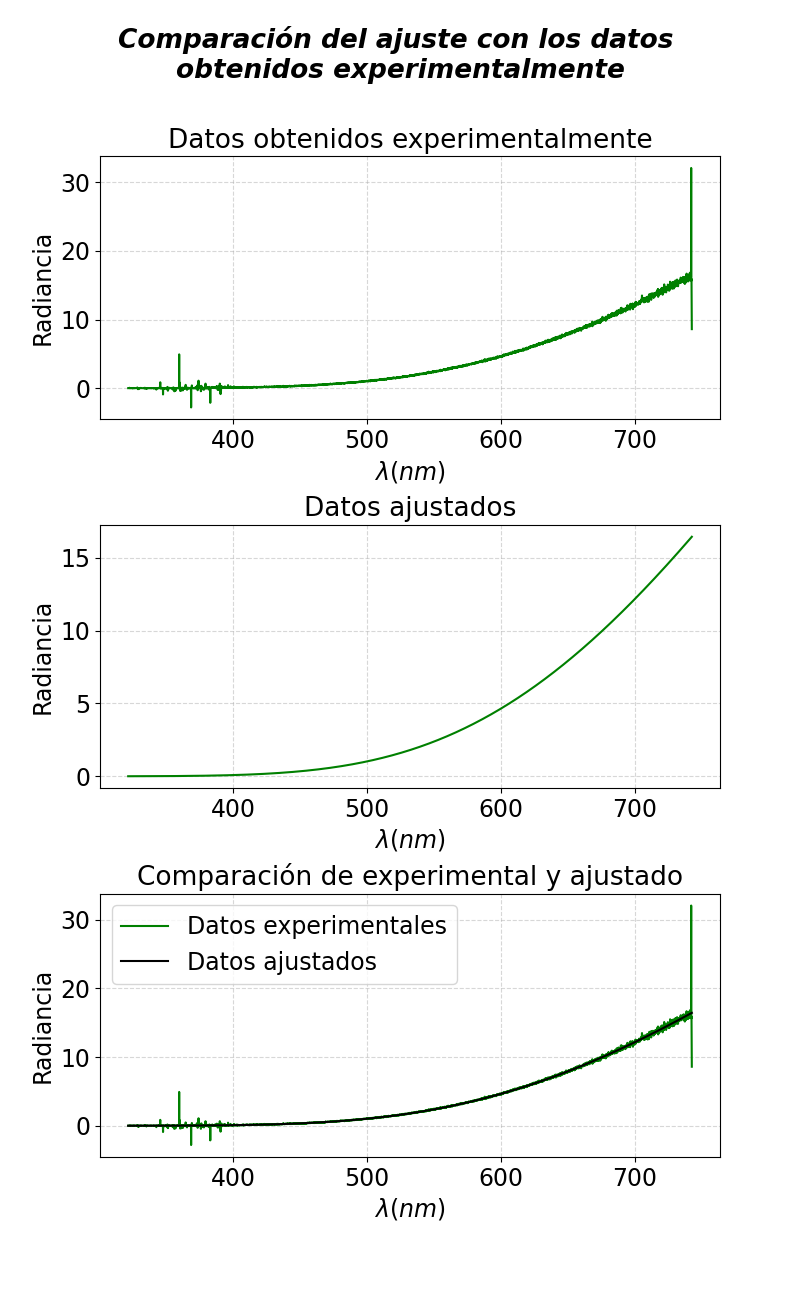
\includegraphics[width =1\linewidth]{Comparación_con_el_ajuste.png}
    \caption{Comparación del ajuste de la ley de Planck con los datos experimentales}
    \label{fig: Ajuste de la ley de planck}
\end{figure}

En la segunda gráfica de la figura \ref{fig: Ajuste de la ley de planck} se muestra el resultado del ajuste de
la ley de Planck al aplicar un ajuste exponencial a la ecuación \ref{eq: Ley de planck}. Del parámetro B del ajuste al despejar $T$, ecuación \ref{eq :temperatura}, y al calcular la incertidumbre por medio de la ecuación \ref{eq: pequeñas incertidumbres}, se obtuvo un valor de:
\begin{equation}
    T = (19.8 \pm 0.2)\times 10^2°K 
    \label{v: temperatura}
\end{equation}


Visualmente, la comparación del ajuste con los datos muestra que el ajuste es bueno. Esto se pudo comprobar mediante el test de Chi-cuadrado.

\subsection{Aplicación del test de $\chi^2$}

\begin{figure}[ht]
     \centering
     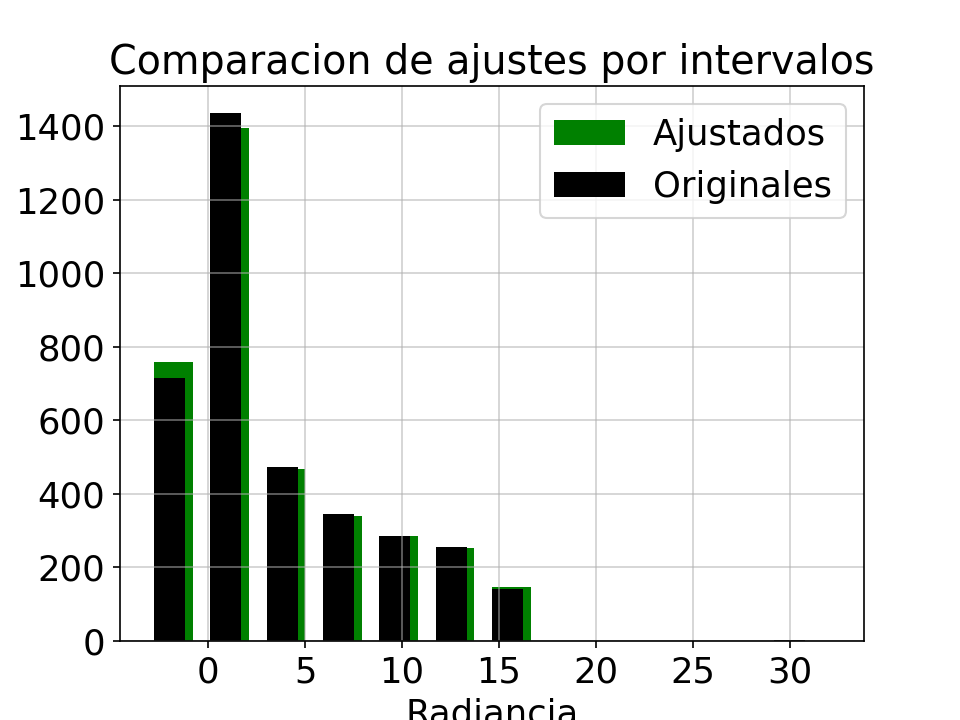
\includegraphics[width =1 \linewidth]{Comparación_con_barras.png}
     \caption{Representación gráfica del número de conteos de intensidades para el test de $\chi^2$}
     \label{fig: aplicación del test}
\end{figure}

En la figura \ref{fig: aplicación del test} se muestra el gráfico de conteos para 12 intervalos de intensidad de los datos ajustados en contraste con los datos obtenidos experimentalmente. Al aplicar el test de $\chi^2$, visto en la sección \ref{seccion chi}, a los conteos obtenidos. Se obtuvo un valor de :
\[
\chi^{2} = 4.13
\]
Se tienen doce bines, acorde a la ecuación \ref{eq: grados de libertad}, el número de grados de libertad corresponden a 9 debido a que se determinaron dos parámetros a partir de los valores experimentales. Luego, $x_*=16.919$ acorde a la figura \ref{fig: valores críticos de chi-cuadrado}. Como $\chi^2<x_*$, se satisface la hipótesis nula, es decir, $H_0:$ \textit{Los datos experimentales siguen la ley de Planck}.

\subsection{Resultados de la ley de Wein}
\begin{figure}
    \centering
    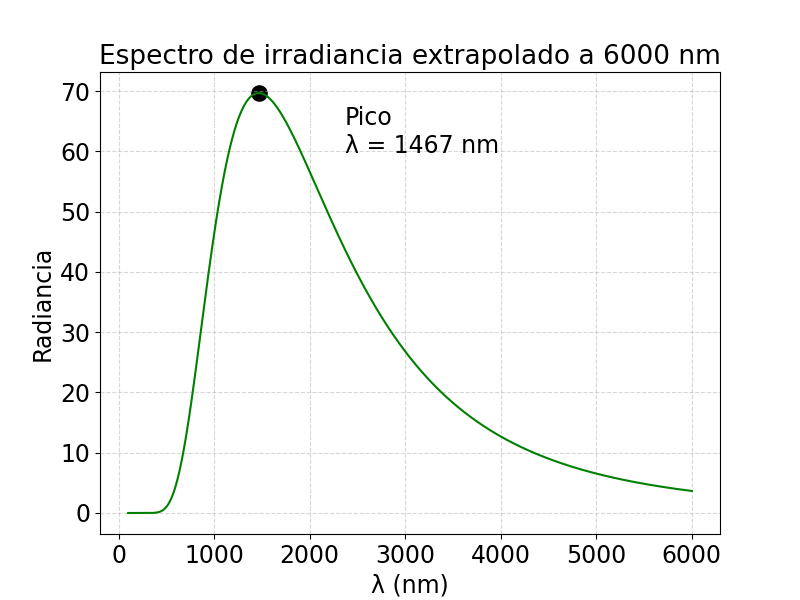
\includegraphics[width= 1\linewidth]{Imagenes/extrapolado.png}
    \caption{Ubicación del pico para el ajuste extrapolado a 6000 nm}
    \label{fig: pico}
\end{figure}
La figura \ref{fig: pico}, muestra los datos de radiancia en función de la longitud de onda, del ajuste mostrado. Extrapolados a 6000 nm, se obtuvó  un valor de $\lambda_{max} = 1467\,nm$. Al usar este valor para encontrar la temperatura, con la ecuación \ref{eq: ley de Wein} :
Se obtuvo:
\[ T = 1976\quad °K\]

Al calcular el error porcentual del  \ref{v: temperatura} en relación con el obtenido con la ley de Wein usando la ecuación \ref{eq: error porcentual}, se obtuvo:  \[\epsilon = 0.2 \% \]

\subsection{Espectros de emisión de distintas lámparas}


En la figura \ref{fig: espectro de emisión} se pueden observar los espectros de emisión de las diferentes fuentes de luz observadas. En la gráfica correspondiente a la lámpara de mercurio - argón se pueden observar los picos de emisión; el primer pico corresponde a un valor de $366.9\,nm$; según la literatura \cite{HG}, este pico pertenece al espectro del mercurio y su valor aceptado es de $365.0158 \,nm$. 

El segundo máximo de $406.5,nm$ pertenece al espectro del mercurio y, según la literatura, su valor aceptado es de $404.6565,nm$. El tercer pico de la gráfica está en $409.7,nm$ y, acorde con la literatura \cite{Argon}, pertenece al espectro de emisión del argón, cuyo valor aceptado es de $404.4418,nm$. El cuarto pico tiene un valor experimental de $437.7,nm$ y un valor aceptado de $435.8335,nm$, correspondiente al espectro de emisión del mercurio. Para el quinto pico, su valor experimental fue de $547.9,nm$ y el valor aceptado de $546.0750,nm$, que nuevamente corresponde al espectro del mercurio. En el sexto se obtuvo un valor experimental de $580.8,nm$ y un valor aceptado de $580.3782,nm$, perteneciente también al espectro del mercurio. Para el séptimo pico se obtuvo un valor experimental de $731.8,nm$, con un valor aceptado de $731.1716,nm$, perteneciente al espectro de emisión del argón. Cabe aclarar que se escogieron esos valores aceptados y el gas al que pertenecían con base en su cercanía al valor experimental y a la intensidad relativa, observando cuál de ambos gases presentaba una mayor intensidad relativa en las cercanías de una longitud de onda determinada.

Para la gráfica de la lámpara LED de la figura \ref{fig: espectro de emisión}, se puede observar un pico en $456.9,nm$, en el rango del azul, y una gran banda entre aproximadamente los $500$ y $600,nm$, lo cual concuerda con lo mostrado en \cite{Ohno2005}. Según este modelo, el fósforo aplicado al LED funciona como un \textit{simulador} del cuerpo negro que sigue la ley de Planck, pero optimizado para una mayor eficiencia luminosa. Esta meseta mencionada entre los $500$ y $600,nm$ sirve para obtener una luz blanca neutra y de buena calidad.
\begin{figure}[H]
    \centering
    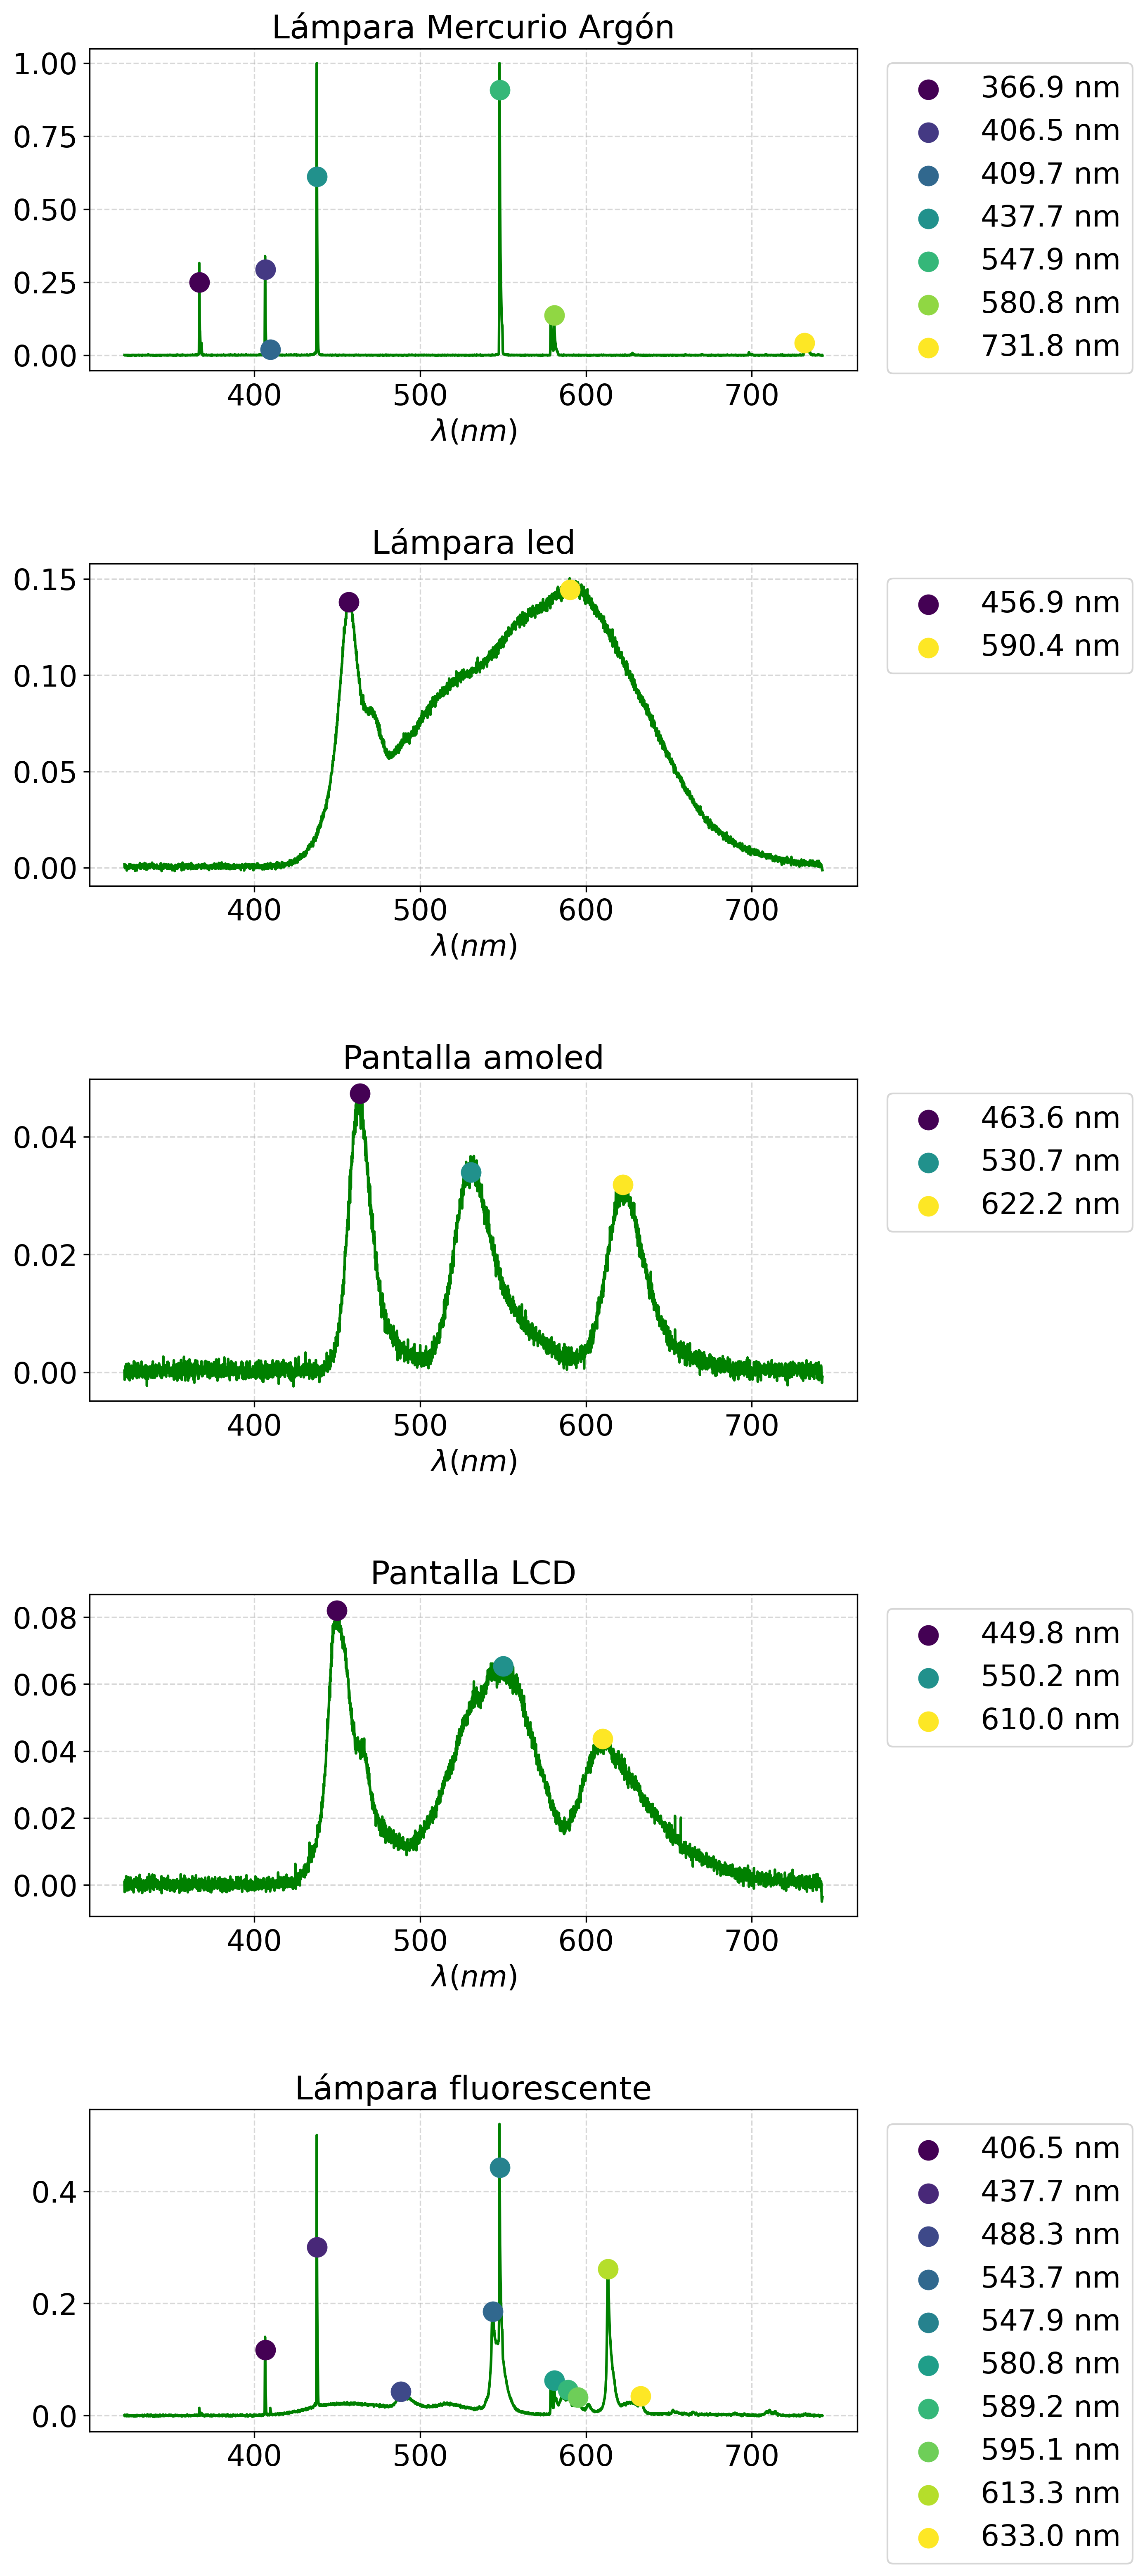
\includegraphics[width=1\linewidth]{Imagenes/espectros_de_otras_lámparas.png}
    \caption{Espectro de emisión de las muestras.}
    \label{fig: espectro de emisión}
\end{figure}

Ahora se procederá a analizar los espectros de emisión de las pantallas AMOLED y LCD de la figura \ref{fig: espectro de emisión}. En primera instancia, y acorde con las secciones 2.7 y 2.8 del \textit{Marco teórico}, se explicó que las pantallas LCD tienen una luz blanca de fondo para iluminar el cristal líquido y darle color a la imagen por medio de polarizadores. En cambio, cada píxel de la pantalla AMOLED tiene su propia fuente de luz. Esto se puede observar en la gráfica, ya que, en comparación, la pantalla AMOLED presenta picos mucho más finos y delineados, lo que implica que, para la pantalla LCD, al tener una fuente de luz de fondo, los polarizadores, por más perfectos que sean, dejan pasar algo de ruido en forma de longitudes de onda no deseadas. Como se mencionó, la pantalla AMOLED tiene picos más finos entre los tres colores primarios (rojo, verde y azul, acorde con la sección \textit{Marco teórico}), por lo cual se obtiene una mayor pureza cromática. Esto implica que los colores están mejor definidos y no se solapan entre sí, permitiendo que la pantalla AMOLED tenga una representación de colores más amplia y precisa. Nótese que, en la gráfica de la pantalla LCD, hay cierto ruido de fondo; es decir, al presentarse un pico, este no cae a cero después del máximo, sino que permanece en una especie de mínimo de intensidad que en la pantalla AMOLED no existe. Esto se debe a que la pantalla LCD tiene una iluminación de fondo, generalmente un LED, que permite visualizar los colores, pero que reduce la fidelidad cromática, especialmente en los tonos negros. Como se mencionó, esos tres picos en ambas pantallas corresponden a los colores primarios rojo, verde y azul, empleados en la formación de imágenes. Idealmente, acorde con \cite{Masaoka2014}, las longitudes de onda para las cuales la representación de los colores es mejor son: para el azul, $467.1,nm$; para el verde, $532,nm$; y para el rojo, $630,nm$. En las gráficas se puede observar que los picos máximos más cercanos a estos valores ideales corresponden a la pantalla AMOLED; en cambio, la LCD cuenta con picos más alejados de dichos valores, lo que implica una peor representación del color.

Para la lámpara fluorescente (figura \ref{fig: espectro de emisión}), se obtuvo que el primer pico significativo fue de $406.5,nm$. Este pico pertenece al espectro de emisión del mercurio y su valor, según la literatura \cite{HG}, es de $404.6565,nm$. El segundo pico fue observado en $437.7,nm$, correspondiente también al espectro de emisión del mercurio, con un valor aceptado de $435.8335,nm$. Para el cuarto pico se obtuvo un valor de $543.7,nm$, correspondiente a una línea del Calcium Tungstate (CAT) \cite{Lamptech2011}, cuyo valor teórico es de $543,nm$. El quinto pico se encontró en $547.9,nm$; esta línea pertenece al espectro del mercurio y cuenta con un valor aceptado de $546.0750,nm$. Ahora se analizará el pico de $613.3,nm$, que según la literatura pertenece al Yttrium Oxide (YOX) \cite{Lamptech2011}, con un valor teórico de $611,nm$. Los picos más hacia la derecha, como el de $633,nm$, pertenecen al espectro de emisión del argón, cuyo valor aceptado es de $630.7657,nm$. En general, el argón presenta picos en esta región del espectro, pero son mucho más pequeños comparados con el resto, debido a que su función principal es ayudar al encendido de la lámpara.

Los picos asociados al fósforo se deben al recubrimiento fluorescente presente en la lámpara, el cual absorbe radiación ultravioleta generada por el mercurio y la reemite en el rango visible. Estos fósforos producen bandas más anchas que las líneas discretas del mercurio debido a los procesos de emisión en materiales sólidos \cite{CAMEOFluorescent}

\section{Conclusiones}
\begin{itemize}
    \item En primer lugar, se pudo verificar experimentalmente la ley de Planck para el cuerpo negro, como se pudo observar en la sección de \textit{Resultados}, los datos experimentales obtenidos se ajustan perfectamente acorde a un ajuste de la forma de la ley de Planck. Lo cual, demuestra la naturaleza discreta de la luz predicha por la teoría cuántica.
    \item Se obtuvo que del ajuste de la ley de Planck, una temperatura de $(19.2\pm0.2)\,K$. Posteriormente, se extrapoló el ajuste hasta los $6000\,nm$ y por medio de la ley de Wein se obtuvo una temperatura de $1976\,K$ lo cual discrepa del ajuste de la ley Plank en un $0.2 \%$, lo cual, indica una coherencia entre ambos métodos de calculo de la temperatura de la lámpara, adicionalmente, del ajuste extrapolado se obtuvo que la longitud de onda donde la radiancia es máxima en$\lambda=1467\,nm$.
    \item Del análisis de los espectros de emisión de las diferentes fuentes se obtuvo que es posible determinar los elementos de los cuales la lámpara está compuesta sabiendo los espectros por separado de cada elemento. Un resultado importante a mencionar en este apartado fue que los espectros de los gases como el mercurio o argón son líneas discretas, como se puede observar en la gráfica de la lámpara de mercurio, en otros casos como los sólidos, particularmente los fósforos de la lámpara de fluorescente, no presentan un espectro discreto sino que tiene un carácter continuo lo que los diferencia de los gases.
    \item En el caso de la lámpara led, se pudo observar que presenta dos picos en los $456.9\,nm$ y $590.4\,nm$, como se explicó en el apartado de \textit{Resultados}, entre los 500 y 600 nanómetros presenta una gran banda estable debido a que el fósforo aplicado para los LEDs funcionan como un \textit{simulador} de cuerpo negro para optimizar la luminosidad, esta meseta se presenta para formar una luz blanca neutra y de una buena calidad.
    \item En el análisis de las pantallas AMOLED y LCD se llegó a la conclusión de que la pantalla AMOLED presenta una mayor fidelidad de los colores debido a sus características, al tener una mayor pureza cromática, se tuvo un espectro menos difuso y un color negro mucho más profundo y real, una mayor pureza cromática indica una mejor representación de los colores que se muestran en la pantalla.
    \item El espectrómetro empleado resultó ser bastante eficaz para nuestro análisis, sin embargo, en varios resultados, difirió del valor real de los espectro en al menos un nanómetro, por lo cual, para un trabajo donde se requiera una máxima precisión del espectro, se recomienda utilizar un espectrómetro más preciso para obtener los resultados deseados.
\end{itemize}

\bibliographystyle{unsrt}
\bibliography{EspectroscopiaNotes}
\appendix
\onecolumn
\begin{center}
    \Large \textbf{Apéndices} % "Large" es un tamaño mediano-grande elegante
\end{center}
\section{Valores Críticos de $\chi^2$}
\begin{figure}[H]
     \centering
     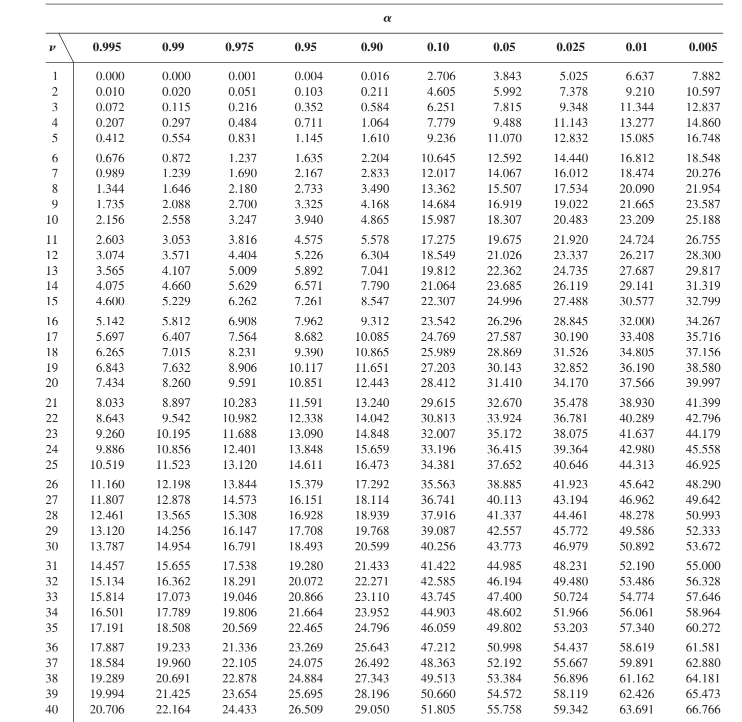
\includegraphics[width =0.7 \linewidth]{Imagenes/valores críticos de chi-cuadrado.png}
     \caption{Valores Críticos de $\chi^2$, tomado de \cite{devore2008}}
     \label{fig: valores críticos de chi-cuadrado}
\end{figure}

\section{Material Complementario}
Se puede acceder al notebook en el que se realizo el análisis de los datos por medio del siguiente enlace:
\url{https://github.com/Jesus-Gamboa/Experimental_IV/blob/main/Espectroscop%C3%ADa/Notebook.ipynb}


\end{document}